\chapter{Filter Modelling} \label{chap:filt}

After defining the glottal pulse shape and the way it is generated, the next logical step is to model the vocal tract. The vocal tract is modeled as an All-Pole Infinite Impulse Response (IIR) filter, which is used to model the spectral envelope of the speech signal. The filter coefficients are estimated using the Linear Predictive Coding (LPC) analysis, which is a method used to model the spectral envelope of the speech signal. The filter coefficients are then used to synthesize the speech signal by exciting the IIR filter with the pulses. These coefficients are estimated using the autocorrelation method, which first estimates the autocorrelation function of the speech signal using the Weiner-Khintchine theorem, and the coefficients are then estimated using the Levinson-Durbin recursion, which is an efficient algorithm that recursively estimates the filter. 

The filter coefficients are then used to synthesize the speech signal using the IIR filter, which is implemented using the direct form II realization. The filter is then used to synthesize the speech signal using the pulse train generated in the previous chapter, on a pulse-by-pulse basis. This meaning that each pulse is used to excite the filter individually before being concatenated as shown in Chapter \ref{chap:pulseGen}.


\section{LPC Analysis}

As introduced previously in Chapter \ref{chap:back}, the Linear Predictive Coding (LPC) analysis is a method used to model the spectral envelope of a signal. For the purpose of this work, the LPC analysis is used to estimate the filter coefficients of an All-Pole Infinite Impulse Response (IIR) filter that models the vocal tract of the speaker. The LPC analysis is performed on the speech signal $x(n)$, which is divided into overlapping frames of length $N_{\text{frame}} = 512$. The LPC analysis is performed on each frame of the speech signal, and the filter coefficients are estimated for each frame. The filter coefficients are then used to synthesize the speech signal using the IIR filter \cite{hayes1996statistical}.

The LPC analysis is performed using the autocorrelation method, which is depicted in Figure \ref{fig:lpcAnalysis}. The autocorrelation method estimates the autocorrelation function of the speech signal through means of the Weiner-Khintchine theorem.

\begin{figure}[H]
    \centering
    \begin{tikzpicture}[auto, node distance=2cm, >=latex']
        \tikzset{
            block/.style = {draw, rectangle, minimum height=3em, minimum width=3em},
            sum/.style = {draw, circle, node distance=1cm},
            input/.style = {coordinate},
            output/.style = {coordinate},
            pinstyle/.style = {pin edge={to-,thin,black}}
        }
        % ODFT 
        \draw (3,-1) rectangle ++(4, 2);
        \node at (5, 1.3) {\it ODFT};

        \node [coordinate] (input) {};
        \node [circle, draw, inner sep = 1pt, right of=input] (mult) {$\times$};
        \node [coordinate, above =0.5cm of mult] (win) {};
        \node [above = 0.1cm of win] (window) {$h[n]$};
        \node [rectangle, minimum width = 1.5cm, minimum height = 1cm,draw, right of = mult] (exp) {$e^{-j\frac{n\pi}{N}}$};
        \node [rectangle, minimum width = 1.5cm, minimum height = 1cm, draw, right of = exp] (dft) {DFT};
        \node [rectangle, minimum width = 1.5cm, minimum height = 1cm, draw, right of = dft] (psd) {$|X[k]|^2$};
        \node [rectangle, minimum width = 1.5cm, minimum height = 1cm, draw, align=center, right = 0.5cm of psd] (lev) {Weiner Khinchine \\ + \\ Levinson Durbin};
        \node [coordinate, right = 2cm of lev] (output) {};
        
        \draw [->] (input) -- node {$x[n]$} (mult);
        \draw [->] (win) -- (mult);
        \draw [->] (mult) -- (exp);
        \draw [->] (exp) -- (dft);
        \draw [->] (dft) -- (psd);
        \draw [->] (psd) -- (lev);
        \draw [->] (lev) -- node {$a_0 \dots a_k$} (output);
    \end{tikzpicture}
    \caption{LPC Analysis Signal Flow Graph}
    \label{fig:lpcAnalysis}
\end{figure}

\subsection{ODFT}

As the filter coefficients are determined in the frequency domain, by means of the Odd Discrete Fourier Transform (ODFT) \cite{ferreiraAccurateEstimationODFT2001}. The Odd Fourier transform is what is referred to as a partial transform, which takes advantage of the property that for a given signal $x(n)$ the Nth order DFT of the signal is real and even, i.e. $X(k) = X(N-k)$, and thus it is only necessary to compute the odd part of the DFT \cite{bellanger2024digital}.

This property is used to both reduce the computational complexity of the DFT algorithm, by only computing the odd part of the DFT of the signal and to achieve perfect signal reconstruction \cite{ferreiraAccurateEstimationODFT2001} when no processing is done between the input and output. Firstly, the transform is computed by multiplying the signal $x(n)$ by a window function $h(n)$, in this case a shifted Sinusoidal window, as shown in Equation \ref{eq:windowFunc}.

\begin{equation}
    h[n] = \sin \left ( \frac{\pi(n+0.5)}{N} \right )
    \label{eq:windowFunc}
\end{equation}

Next, this operation is followed by then multiplying the result by the exponential function $e^{-j\frac{n\pi}{N}}$. The ODFT is then finally computed using a standard FFT algorithm, and the power spectral density of the speech signal is estimated resulting in what is sometimes referred to as the Power ODFT \cite{goncalvesVozeamentoSinteticoVoz2023}.



%The ODFT is a method used to estimate the Discrete Fourier Transform (DFT) of a signal using the autocorrelation function of the signal. The ODFT is used to estimate the DFT of the speech signal $x(n)$, which is then used to estimate the filter coefficients of the IIR filter. The ODFT is performed on the speech signal $x(n)$, which is multiplied by a window function $sinW(n)$, and then multiplied by the exponential function $e^{-j\frac{n\pi}{N}}$. The ODFT is then computed using the DFT algorithm, and the power spectral density of the speech signal is estimated. The Weiner-Khintchine theorem is then used to estimate the autocorrelation function of the speech signal, which is then used to estimate the filter coefficients using the Levinson-Durbin recursion.

\subsection{Levinson-Durbin algorithm}

The Levinson-Durbin recursion is an efficient algorithm that recursively estimates the filter coefficients by minimizing the prediction error \cite{yuMultistageLevinsonDurbinAlgorithm2002}. The filter coefficients are estimated by solving the Toeplitz system of Equations (\ref{eq:yulewalker}) presented in Chapter \ref{chap:back}, which require the autocorrelation coefficients of the speech signal to first be determined by means of the Weiner-Khintchine theorem. The algorithm has a time complexity of $O(n^2)$ \cite{hayes1996statistical}, whereas other methods of solving the required system of equations, say through a least squares approach, would have a time complexity of $O(n^3)$. 
\begin{comment}
A general description of the Levinson-Durbin recursion is as follows \cite{yuMultistageLevinsonDurbinAlgorithm2002}:

\begin{enumerate}
    \item Determine the autocorrelation sequence \( r[\tau] \)
    \item Initialize \( E_0 = r[0] \), \( a_0 = 1 \)
    \item For \( i = 1, 2, \ldots, p \):
    \begin{enumerate}
        \item Calculate the reflection coefficient (also known as the Parcor coefficient):
        \[
        k_i = \frac{r[i] - \sum_{j=1}^{i-1} a_j^{(i-1)} r[i-j]}{E_{i-1}}
        \]
        \item Update the prediction error:
        \[
        E_i = (1 - k_i^2) E_{i-1}
        \]
        \item Update the coefficients:
        \[
        a_i = a_{i-1}^{(i-1)} + k_i \left( 1 - \sum_{j=1}^{i-1} a_j^{(i-1)} \right)
        \]
        \item For \( j = 1, 2, \ldots, i-1 \):
        \[
        a_j^{(i)} = a_j^{(i-1)} - k_i a_{i-j}^{(i-1)}
        \]
    \end{enumerate}
\end{enumerate}
\end{comment}

The Levinson-Durbin recursion is implemented in Python in listing \ref{lst:levinsonPy}, and is written taking advantage of the vector and matrix processing capabilities that are provided by NumPy. The function \texttt{levinson()} takes as input the autocorrelation coefficients $r$ of the speech signal and the filter order $N$, and returns the filter coefficients $a[k]$, the prediction error $E$, and the reflection coefficients $k$.

Besides the calculation of the $a_k$ filter denominator coefficient, another important metric is that of the $b_0$ filter gain coefficient. This coefficient is calculated as the square root of the prediction error $E$. This is called the autocorrelation matching property, and it is used to ensure that the energy of input signal is the same as the energy of the filter which is given by its first autocorrelation coefficient \cite{hayes1996statistical}.

\begin{lstlisting}[language=Python, style=mystyle, caption={Levinson Durbin Recursion in Python}, label={lst:levinsonPy}]
    def levinson(r, N):
        k = np.zeros(N+1) # Reflection coefficients
        A = np.zeros(N+1) # Prediction filter coefficients
        A[0] = 1.0
        E = np.real(r[0]) # Prediction error
    
        # Levinson-Durbin recursion
        for i in range(1, N+1):
            lambda_ = -np.dot(r[1:i+1], A[i-1::-1]) / E
            A[1:i+1] += lambda_ * A[i-1::-1]
            E *= (1.0 - lambda_ * lambda_)
            k[i] = -lambda_  # Reflection coefficient is the negation of lambda_
        
        return A, E, k[1:]
    \end{lstlisting}

Before applying the Levinson-Durbin algorithm for the estimation of the filter coefficients, the autocorrelation coefficients of the speech signal must be estimated. The autocorrelation coefficients are estimated using the Weiner-Khintchine theorem, which states that the autocorrelation function of a signal is the inverse Fourier transform of the power spectral density of the signal \cite{hayes1996statistical, engelberg2006random}. The power spectral density of the speech signal is estimated using the ODFT, and the autocorrelation coefficients are then estimated using the inverse Fourier transform of the power spectral density. For an input signal $x[n]$ with a corresponding ODFT of $X[k]$, the autocorrelation coefficients $r[\tau]$ are estimated using the Weiner-Khintchine theorem as shown in Equation \ref{eq:wienerkhintchine}, where $\mathcal{F}^{-1}$ represents the inverse ODFT operation and $PSD[k]$ is the Power Spectral Density corresponding to signal $x[n]$.

\begin{equation}
    r[\tau] = \mathcal{F}^{-1}\{|X[k]|^2\} = \mathcal{F}^{-1}\{PSD[k]\}
    \label{eq:wienerkhintchine}
\end{equation}

\subsubsection{Realtime Implementation}

The Levinson-Durbin recursion is implemented in C in listing \ref{lst:levinsonC}. The function \texttt{levinson()} takes as input the autocorrelation coefficients $r$ of the speech signal and the filter order \texttt{n}, and returns the filter coefficients \texttt{a}, the prediction error \texttt{e}, and the reflection coefficients \texttt{k}.

\begin{lstlisting}[language=C, caption={Levinson Recursion in C}, label={lst:levinsonC}]
void levinson(float32_t* r, uint16_t n_len, float32_t* a, float32_t* e){
    float32_t lambda[n_len + 1];
    a[0] = 1.0;
    *e = r[0];

    float32_t lambdaSum, temp;
    for (size_t i = 1; i <= N; i++){
        lambdaSum = 0.0f;

        for (size_t j = 1; j <= i; j++)
            lambdaSum += a[j] * r[i - j];

        lambda[i] = -lambdaSum / (*e);

        for (size_t j = 1; j <= i / 2; j++){
            temp = a[j] + lambda[i] * a[i - j];
            a[i - j] += lambda[i] * a[j];
            a[j] = temp;
        }

        a[i] = lambda[i];
        (*e) = (*e) * (1 - lambda[i] * lambda[i]);
    }

    return;
}
\end{lstlisting}


\section{Filter Realization}

The standard formula for the IIR filter response in the z-domain is given by Equation (\ref{eq:typeIIfilter}). The filter coefficients $a_k$ and $b_0$ are determined by the LPC analysis, and the filter order $N$ is determined by the number of poles in the LPC analysis.

\begin{equation}
    H(z) = \frac{B(z)}{A(z)} = \frac{b_0 + \sum_{k=1}^{N}b_k z^{-k}}{1 + \sum_{k=1}^{N}a_k z^{-k}}
    \label{eq:typeIIfilter}
\end{equation}

In order to implement the IIR filter, we need to choose a realization structure. The direct form II realization is chosen for its simplicity and ease of implementation, as only single delay line $w(n)$ is needed and no reflection coefficients need to be computed \cite{jackson1996digital}. The signal flow chart for this type of realization is shown in Figure \ref{fig:directTypeII} for a second order system. Considering the input signal $x(n)$ and the output signal $y(n)$, the direct form II realization of the IIR filter can be described by the following difference equations in \ref{eq:directTypeII}.

\begin{equation}
    \begin{cases}
        w(n) = x(n) - \sum_{k=1}^{N} a_k w(n-k) \\
        y(n) = \sum_{k=0}^{N} b_k w(n-k) = b_0 w(n)
    \end{cases}
    \label{eq:directTypeII}
\end{equation}


\begin{figure}[H]
    \centering    

    % direct type II IIR realization tikz picture
    \begin{tikzpicture}[auto, node distance=2cm,>=latex']
        % Nodes
        \node [coordinate] (input) {};
        \node [circle, draw, inner sep=1pt, right of=input] (sum1) {$+$};
        \node [coordinate, right of=sum1, label = above:$w(n)$] (delay0) {};
        \node [rectangle, draw, below = 0.75cm of delay0] (delayLine1) {$z^{-1}$};
        \node [coordinate, below=0.75cm of delayLine1] (delay1) {};
        \node [rectangle, draw, below= 0.75cm of delay1] (delayLine2) {$z^{-1}$};
        \node [coordinate, below=0.75cm of delayLine2] (delay2) {};    
        \node [isosceles triangle, draw, right=1cm of delay0, label = above:$b_0$] (b0) {};
        \node [isosceles triangle, draw, right=1cm of delay1, label = above:$b_1$] (b1) {};
        \node [isosceles triangle, draw, right=1cm of delay2, label = above:$b_2$] (b2) {};
        \node [isosceles triangle, rotate=180, draw, left=1.2cm of delay2, label = below:$-a_2$] (a2) {};
        \node [isosceles triangle, rotate=180, draw, left=1.2cm of delay1, label = below:$-a_1$] (a1) {};
        \node [circle, draw, inner sep=1pt, left=1.15cm of a1] (sum2) {$+$};
        \node [circle, draw, inner sep=1pt, right=0.7cm of b1] (sum3) {$+$};
        \node [circle, draw, inner sep=1pt, right=0.7cm of b0] (sum4) {$+$};
        \node [coordinate, right of = sum4] (output) {};

        % Connections
        \draw [->] (input) -- node {$x(n)$} (sum1);
        \draw [-] (sum1) -- (delay0);
        \draw [->] (delay0) -- (delayLine1);
        \draw [->] (delay0) -- (b0);
        \draw [-] (delayLine1) -- (delay1);
        \draw [->] (delay1) -- (b1);
        \draw [->] (delay1) -- (a1);
        \draw [->] (delay1) -- (delayLine2);
        \draw [-] (delay2) -- (delayLine2);
        \draw [->] (a1) -- (sum2);
        \draw [->] (a2) -- ++(-1.25cm, 0) -- (sum2);
        \draw [->] (delay2) -- (a2);
        \draw [->] (delay2) -- (b2);
        \draw [->] (sum2) -- (sum1);
        \draw [->] (b0) -- (sum4);
        \draw [->] (b1) -- (sum3);
        \draw [->] (sum4) -- node {$y(n)$} (output);
        \draw [->] (sum3) -- (sum4);
        \draw [->] (b2) -- ++(1.42cm, 0) -- (sum3);
    \end{tikzpicture}
    
    \caption{Direct-Type-II IIR Filter Signal Flow Graph - 2nd order}
    \label{fig:directTypeII}
\end{figure}

\subsection{Realtime Implementation}

The structure represented in figure \ref{fig:directTypeII} is, obviously, simplified and in our implementation its order is determined by the number of poles in the LPC analysis. It is also worth to note that all filter numerator coefficients besides $b_0$ are all null. Therefore, there is room to reduce the computational complexity of the filter.

\begin{lstlisting}[language=C, style=mystyle]
void iirDirectTypeII(float32_t* in, float32_t* out, int len, float32_t b0, float32_t* a, int coeffLen){
    // set output to all zeros
    memset(out, 0.0f, len);
    
    // variable length arrays are allowed in C99
    float32_t w[coeffLen]; // delay line initialized to all zeros
    memset(w, 0.0f, coeffLen);

    for (int32_t i = 0; i < len; i++){
        // First difference equation is to determine w[n] from the denominator
        w[0] = in[i];
        for(int32_t j = 1; j < coeffLen; j++) // compute the output delay line
            w[0] -= a[j] * w[j];

        // Second difference equation is simplified as there is only b0
        out[i] = b0 * w[0];

        // Shift delay line
        for (int32_t j = coeffLen - 1; j > 0; j--)
            w[j] = w[j - 1];
    }

    return;
}    
\end{lstlisting}


\section{Spectral Tilt Compensation}

One important aspect of the vocal tract filter model is that of the spectral tilt compensation. Tilt compensation is a technique used to adjust the gain of the filter in order to compensate for what is called the spectral tilt of the speech signal \cite{ferreira2018on}. The spectral tilt of the speech signal is a characteristic of the speech signal that is related to the power spectral density of the glottal source signal across the frequency spectrum. It is an important characteristic of the speech signal that can affect the perceived naturalness and quality of the synthesized speech signal. Thus, compensation is required in order to adjust the frequency response of the filter that is inferred from the whispered signal as to improve the quality of the synthesized speech signal.

Using the LF glottal derivate model harmonics that were obtained in Chapter \ref{chap:pulseGen}, the spectral tilt of the glottal pulse can be estimated for any given fundamental frequency. This spectral tilt of the glottal pulse is then used to estimate the spectral tilt of the synthesized speech signal, given the target fundamental frequency. In Figure \ref{fig:tiltGain} we can see the magnitude of the glottal pulse frequency response and how it can be seen rolling off in the higher frequencies. 

\begin{figure}[H]
    \centering
    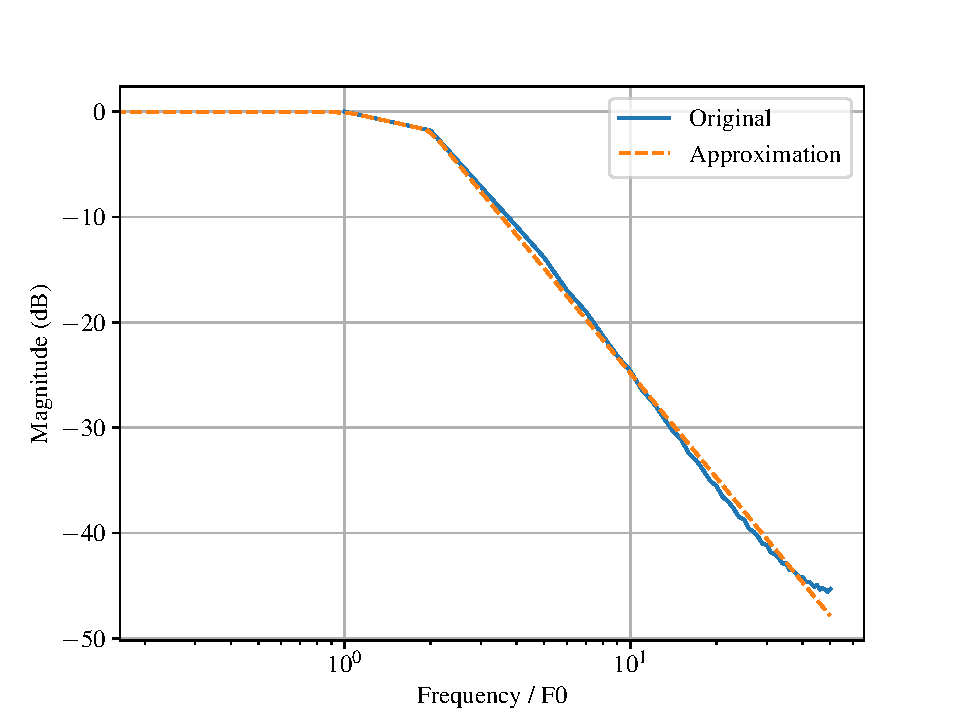
\includegraphics[width = 0.8\textwidth]{chapter5/glottalPulseTiltGain.pdf}
    \caption{Glottal Pulse Spectral Tilt}
    \label{fig:tiltGain}
\end{figure}

In \cite{ferreira2018on}, Ferreira establishes that the spectral tilt compensation can be approximated by a piecewise function consisting of 3 linear segments in the log-frequency domain. The first segment is a flat response, the second segment is a linear increase in gain, and the third segment is a further linear decrease in gain. In this case, the pulse gain is modelled in the following way:

\begin{equation}
    \begin{cases}
        1.0 & \text{if } f < f_0 \\
        b_1 - m_1f & \text{if } f/f_0 \in [1, 2] \\
        b_2 - m_2f & \text{otherwise}
    \end{cases}
\end{equation}

These values are then precomputed at the start of the program and stored in an array that is multiplied to each PSD before doing the IODFT and the Levinson-Durbin recursion. This is done in order to avoid having to do the same calculations over and over for each frame of the speech signal. It is relevant to point out that this function does obviously vary with the fundamental frequency of the glottal pulses, as can be seen in Figure \ref{fig:tiltCompensation}. This effect is noticeable for large variations of $F_0$, but it was deemed as small enough for the microvariations of $F_0$ which most likely do not warrant for this compensation to be computed individually for each pulse period.

\begin{figure}[H]
    \centering
    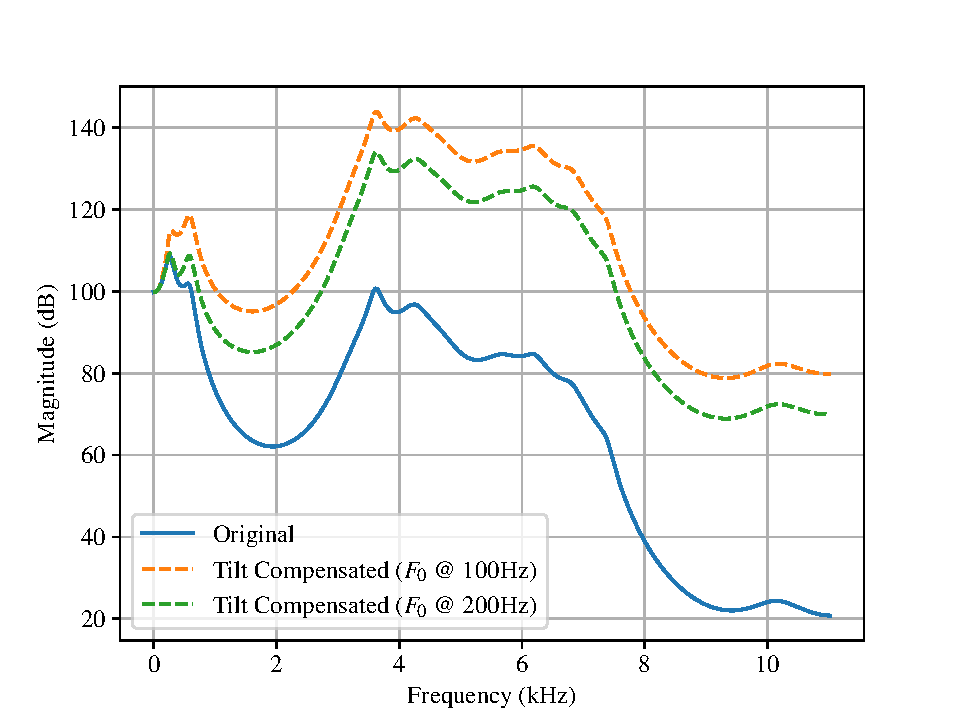
\includegraphics[width = 0.8\textwidth]{chapter5/vowelTiltCompensation.pdf}
    \caption{Comparison of uncompensated and tilt compensated spectral envelopes}
    \label{fig:tiltCompensation}
\end{figure}

\section{Vowel Synthesis}

In order to both validate the filter realization and the tilt compensation, synthetic vowels were generated from a set of vowel spectral envelopes that were determined in a similar fashion to \cite{ferreiraMismatchPhaseStructure2024}, which in turn is based on the LPC estimation mechanism of Figure \ref{fig:lpcAnalysis}. These were inferred before from voiced samples of a very high pitch female voice.

Utilizing the LPC modelling mechanism along with the tilt compensation, filters were generated from each of the vowel spectral envelopes, which were then excited using the LF pulse train generated in Chapter \ref{chap:pulseGen}, following the $F_0$ contour that was established in the same chapter in Equation (\ref{eq:f0Contour}). As determined in previous research on the DyNaVoiceR project \cite{oliveiraModelizacaoFiltroTrato2020} the filter order that was utilized for modelling the vocal tract was $N_{LPC} = 22$, which allows for up to 11 formant frequencies to be represented. Figure \ref{fig:vowelTemplates} shows the spectral envelopes of each of the tonic vowels of European Portuguese, which were used to generate the synthetic vowels.

\begin{figure}[H]
    \centering
    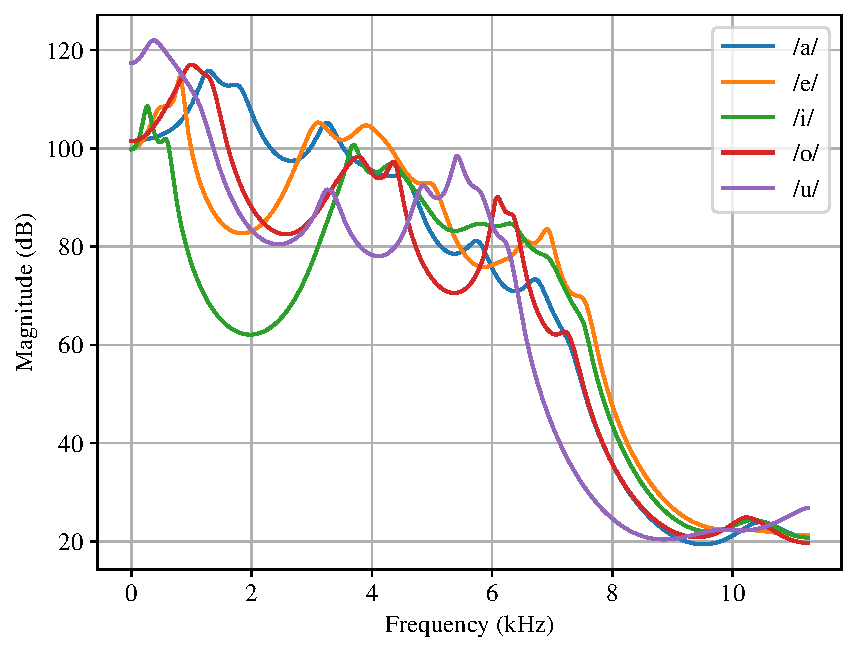
\includegraphics[width=0.7\textwidth]{chapter5/vowelsTemplates.pdf}
    \caption{Spectral envelopes for each tonic vowel of EP}
    \label{fig:vowelTemplates}
\end{figure}

From these spectral envelopes the models are generated using the same LPC analysis mechanism in the previous sections of this chapter. The filters are then excited using a pulse train generated from the LF glottal pulse model that is shown in Chapter (\ref{chap:pulseGen}). The implementation in C can be seen in listing \ref{lst:vowelSynth}, where CMSIS function are taken advantage of in order to speed up not only the computations, as they are optimized for the ARM Cortex-M7 core Neon instructions, but also speed up the development process. 

Regarding the code snippet in \ref{lst:vowelSynth}, the PSD of each vowel was already in memory in the variable \texttt{psd} such that the IODFT can be computed directly, and then Levinson-Durbin recursion is then applied to the reflection coefficients, without analyzing any of the input signal frames coming from the DMA. This is done just for the sake of simplicity, as the main goal of this chapter is to show the filter realization and the tilt compensation mechanism. Figure \ref{fig:vowelPulses} shows the filtered pulses that were obtained in real-time using the spectral envelopes template of the /a/ vowel. 

\mybreak 

\begin{figure}[H]
    \centering
    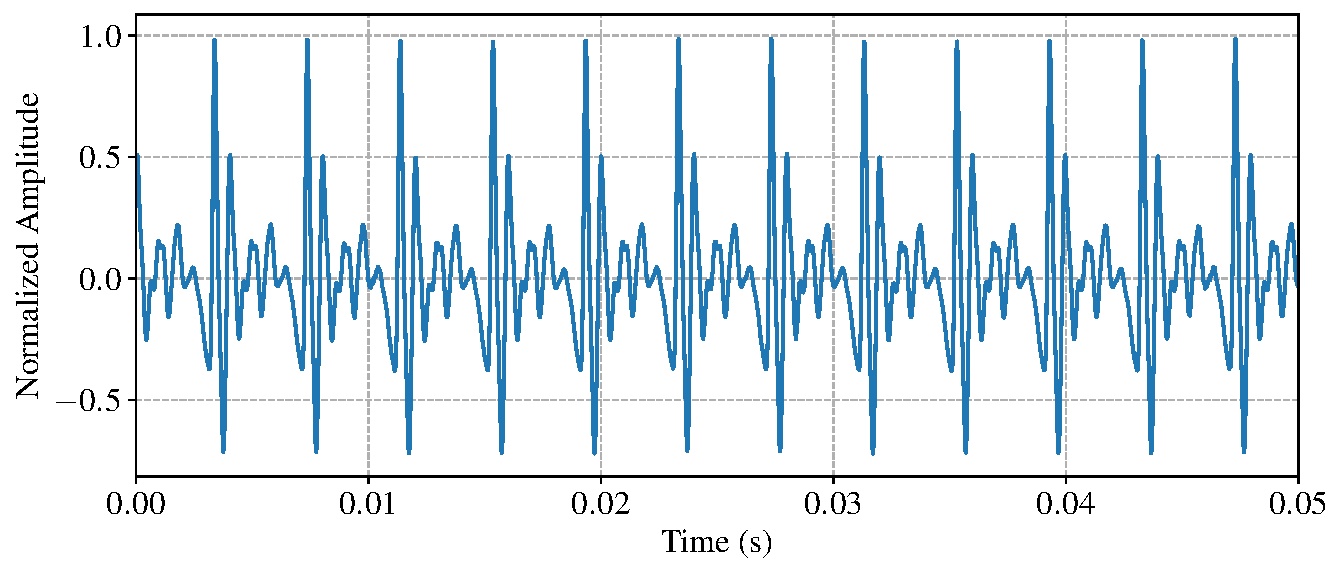
\includegraphics[width=0.9\textwidth]{chapter5/filteredPulses.pdf}
    \caption{Filtered Pulses in realtime}
    \label{fig:vowelPulses}
\end{figure}

Furthermore, the spectral envelopes of the synthetic vowels were also analyzed in order to validate the filter realization and the tilt compensation, in both the Python and realtime environments. Figure \ref{fig:vowelSpectrum} shows the spectral envelope of the ideal synthesized vowel and the synthetic vowel generated using the filter realization and the tilt compensation. The synthetic vowel closely resembles the ideal vowel, which validates the filter realization and the tilt compensation mechanism. 

It becomes clear although that the STM32 is not able to generate the same quality of the synthetic vowels as the Python implementation, which is expected due to not only the computational limitations of the microcontroller that have been exposed in the previous chapter, but also due to the fact that there is a real noise floor on the microcontroller's audio output which is obviously not present in the validation environment.

\begin{figure}[H]
    \centering
    \begin{minipage}[H]{0.495\textwidth}
        \centering
        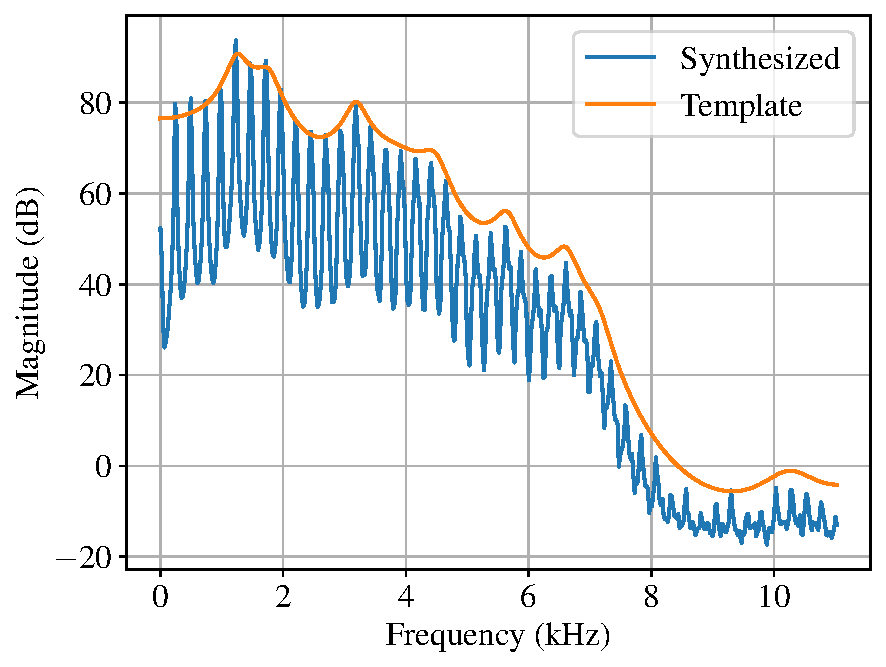
\includegraphics[width=\textwidth]{chapter5/idealSpectrum.pdf}
        \subcaption{}
    \end{minipage}
    \begin{minipage}[H]{0.495\textwidth}
        \centering
        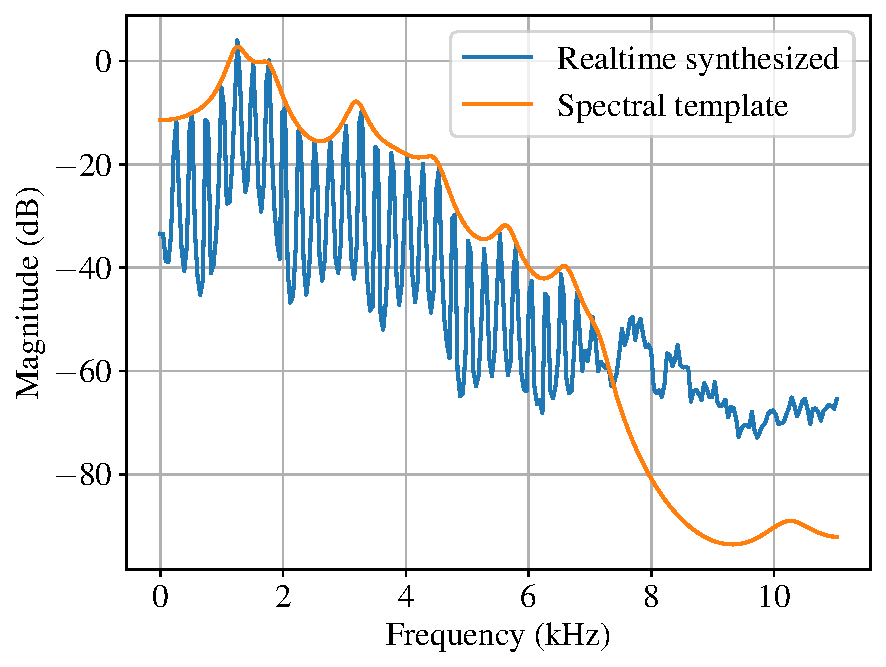
\includegraphics[width=\textwidth]{chapter5/realtimeSpectrum.pdf}
        \subcaption{}
    \end{minipage}
    \caption{Spectral envelope of the ideally synthesized vowel (a) and the realtime synthesized vowel (b)}
    \label{fig:vowelSpectrum}
\end{figure}



%\vspace*{12mm}
